% Created 2020-05-01 Fri 17:01
% Intended LaTeX compiler: pdflatex
\documentclass[12pt]{report}
\usepackage[utf8]{inputenc}
\usepackage[T1]{fontenc}
\usepackage{graphicx}
\usepackage{grffile}
\usepackage{longtable}
\usepackage{wrapfig}
\usepackage{rotating}
\usepackage[normalem]{ulem}
\usepackage{amsmath}
\usepackage{textcomp}
\usepackage{amssymb}
\usepackage{capt-of}
\usepackage{hyperref}
\setlength{\parindent}{0pt}
\usepackage[margin=1in]{geometry}
\usepackage{emptypage}
\usepackage{tikz}
\usetikzlibrary{graphs,graphs.standard,bayesnet,arrows.meta,shapes.arrows}

% Colorlinks sets pdfborder to zero.
%\hypersetup{colorlinks,linkcolor=,urlcolor=gray}

%\usepackage[a4paper,top=2.25cm,bottom=2.25cm,left=3.0cm,right=3.0cm]{geometry}

%% arial font?????????
%% \usepackage[scaled]{uarial}
%% \renewcommand*\familydefault{\sfdefault} %% Only if the base font of the document is to be sans serif
%% \usepackage[T1]{fontenc}

\makeatletter
\renewenvironment{abstract}{%
    \if@twocolumn
      \section*{\abstractname}%
    \else %% <- here I've removed \small
      \begin{center}%
        {\bfseries \Huge\abstractname\vspace{\z@}}%  %% <- here I've added \Large
      \end{center}%
      \quotation
    \fi}
    {\if@twocolumn\else\endquotation\fi}
\makeatother

%\pagecolor{yellow!10}

\documentclass{book}
\usepackage{sectsty}
\chapternumberfont{\large} 
\chaptertitlefont{\huge}

\usepackage{hyperref}
\hypersetup{%
  colorlinks=false,% hyperlinks will be black
  linkbordercolor=red,% hyperlink borders will be red
  pdfborderstyle={/S/U/W 1}% border style will be underline of width 1pt
}

%% \usepackage[T1]{fontenc}
%% \usepackage{libertine}
%% \usepackage{graphicx}
%% \usepackage[svgnames]{xcolor}
%% \usepackage{framed}

%% \newcommand*\openquote{\makebox(25,-22){\scalebox{5}{``}}}
%% \newcommand*\closequote{\makebox(25,-22){\scalebox{5}{''}}}
%% \colorlet{shadecolor}{Azure}

%% \makeatletter
%% \newif\if@right
%% \def\shadequote{\@righttrue\shadequote@i}
%% \def\shadequote@i{\begin{snugshade}\begin{quote}\openquote}
%% \def\endshadequote{%
%%   \if@right\hfill\fi\closequote\end{quote}\end{snugshade}}
%% \@namedef{shadequote*}{\@rightfalse\shadequote@i}
%% \@namedef{endshadequote*}{\endshadequote}
%% \makeatother
%% \begin{document}


\author{Louis James}
\date{\today}
\title{A system for exploring haptic and spatial interaction}
\hypersetup{
 pdfauthor={Louis James},
 pdftitle={A system for exploring haptic and spatial interaction},
 pdfkeywords={},
 pdfsubject={Final year project for Creative Computing},
 pdfcreator={Emacs 26.3 (Org mode 9.3.6)}, 
 pdflang={English}}
\begin{document}

\maketitle
\renewcommand{\abstractname}{Acknowledgements}
\begin{abstract}
 Thanks to my family, Florent, Chudleigh dwellers, Jamie ...
\end{abstract}
\newpage

\renewcommand{\abstractname}{Abstract}
\begin{abstract}
This project\ldots{}
\end{abstract}
\tableofcontents
\listoffigures
\chapter{Introduction}
\label{sec:org41d9406}
\chapter{Background}
\label{sec:orgf25dcaa}

The motivation for this project stems in part from a feeling of frustration in
how working on computers can often be a constricted affair and a pondering over
how we might expand the \emph{keyboard-mouse-monitor} model to improve the utility of
computers regarding our own perceptive abilities. How might a spatial and more
\emph{haptic} environment for interaction create an improved space for thinking with
computers as well as our physical health.

\section{Definitions}
\label{sec:org6cd57f5}
\begin{enumerate}
\item Computing
\label{sec:orgc9a1233}
\item keyboard-mouse-monitor model (kmm model) (?)
\label{sec:orga811450}
\end{enumerate}

\section{Beginning with the Exocortex}
\label{sec:org79f4dcb}

I started off looking at \emph{Exocortexes} and other personal archiving systems.
Systems that allow the user to externalise thought and memory. This could be via
simply storing and organising work and ideas efficiently and methodically or
unifying many tasks or different workflows into a singular interface. \\

Org mode is a good example of such a system. Org mode is a "computing
environment for authoring mixed natural and computer language documents"
\cite{Schulte:Davison:Dye:Dominik:2011:JSSOBK:v46i03}. It is designed for taking
notes, producing documents and organising and runs inside of the text editor,
Emacs. It has the ability to export to different formats such as HTML, \LaTeX{} and
supports "outlining, note-taking, hyperlinks, spreadsheets, TODO lists, project
planning, GTD" as well as literate programming
\cite{Schulte:Davison:Dye:Dominik:2011:JSSOBK:v46i03}.

\begin{itemize}
\item org mode
\item nataniev ecosystem
\end{itemize}

\section{Dynamicland}
\label{sec:orgd3cc1be}

One of my original points of reference was \emph{Dynamicland}, a research project in
Oakland, USA. The aim of the project is to implement a new more powerful and
accessible model of computing.

\begin{quote}


In Oakland, we built the first full-scale realization of the vision, inviting
thousands of people into our space to collaborate. Together, these artists,
scientists, teachers, students, programmers, and non-programmers created
hundreds of projects that would have been impossible anywhere else.
-- Dynamicland.org 
\end{quote}


\emph{Dynamicland} is a communal computer where the building is the computer (ENIAC).
Programs are embodied in the room on pieces of colour-coded paper. The programs
are recognised via the codes and their code, stored in a database is then run,
it can also \emph{read} code using OCR but generally the code is there \href{https://thenewstack.io/dynamicland-rethinks-computer-interfaces/}{symbolically}.
Projectors on the ceiling transform the paper and workbenches into whatever the
programmer decides. This relatively simple model makes for an exciting new
ecosystem for collaborative computing and expressive programming. Victors,
highlights his ideas for the progression of computing and interaction in a
series of talks (available online) and on his \href{http://worrydream.com}{website}. In his talk "Seeing
Spaces" he talks of a new kind of maker-space which allow makers to see across
time and possibilities. \emph{Dynamicland} offers a computational medium which allows
for full use of the human senses for the exploration with of "\href{https://vimeo.com/115154289}{humane
representation[s] of thought}". \cite{VictorKayDynamicLand} \\


\begin{figure}[htbp]
\centering
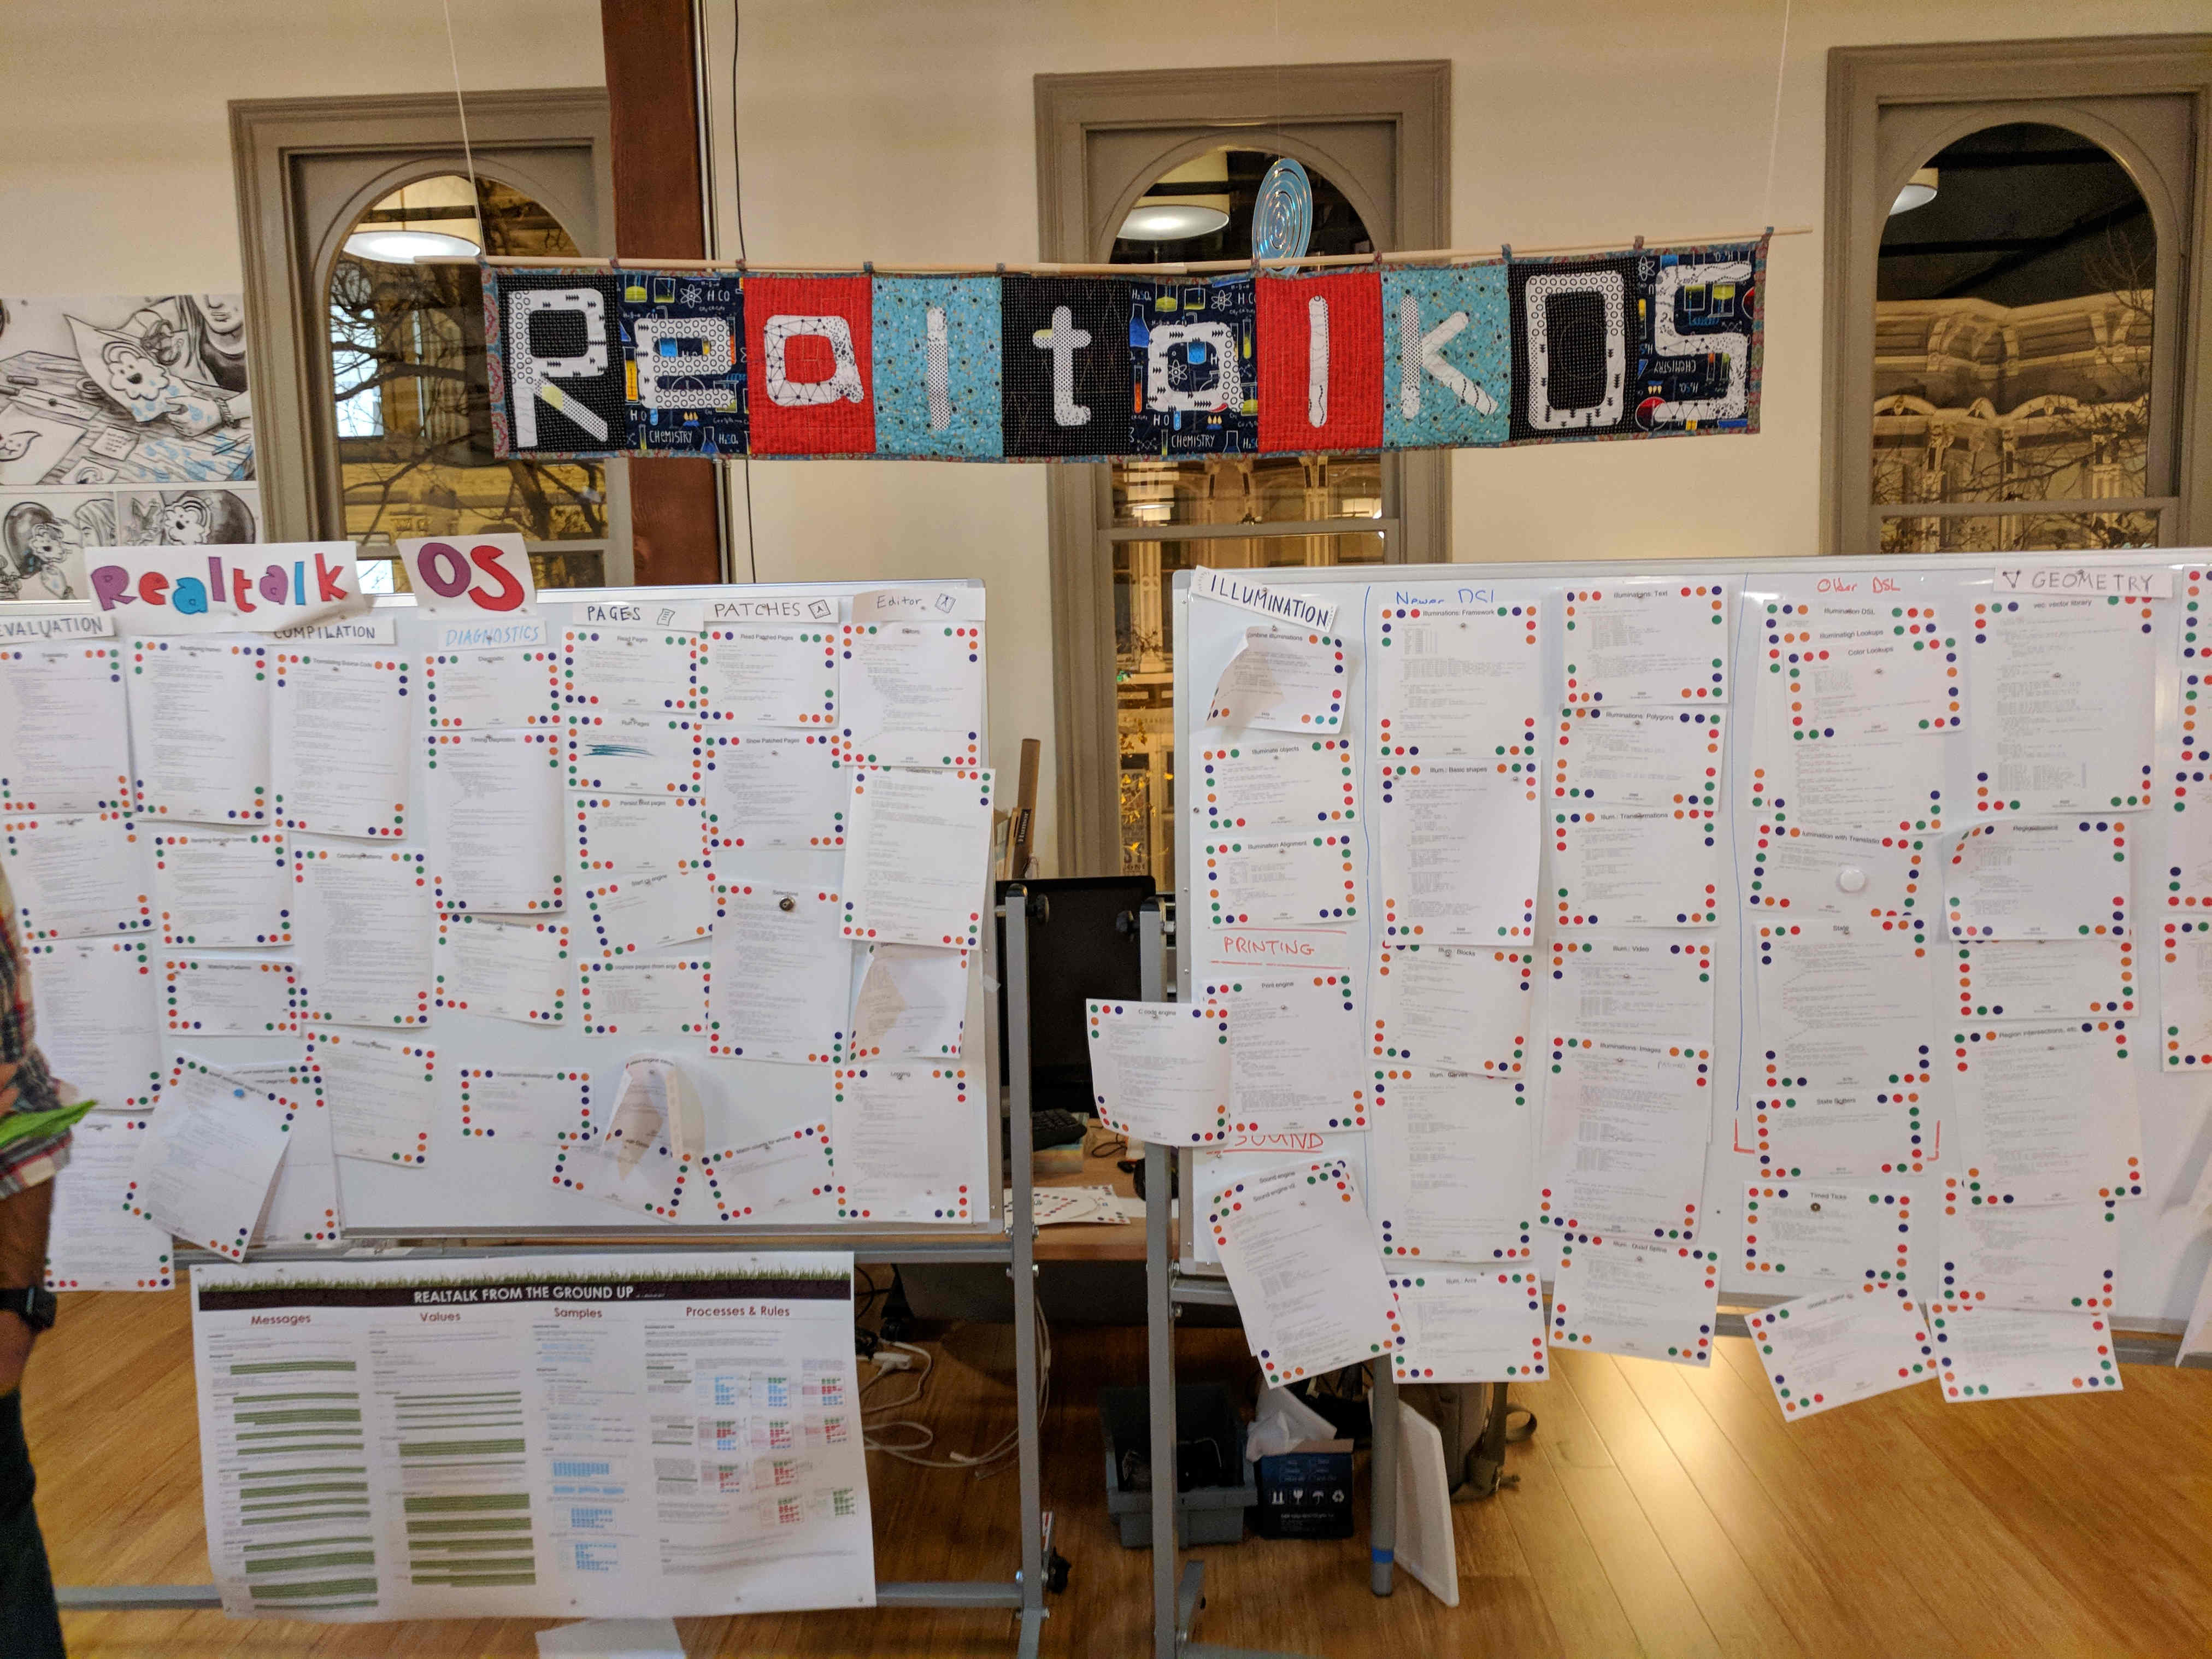
\includegraphics[width=15cm]{assets/realtalk-os.jpg}
\caption{RealtalkOS, the operating system of Dynamicland}
\end{figure} 

\emph{Dynamicland} was the inspiration for the main physical and technical model for
this project, an \emph{augmented} workspace either on the floor or a table which is
projected onto. A camera/s pointing down onto the projection space is the sensor
for detecting interaction, with the projector as the actuator. This model can be
seen in the Figure \ref{pp-schema} .

\begin{figure}[htbp]
\centering
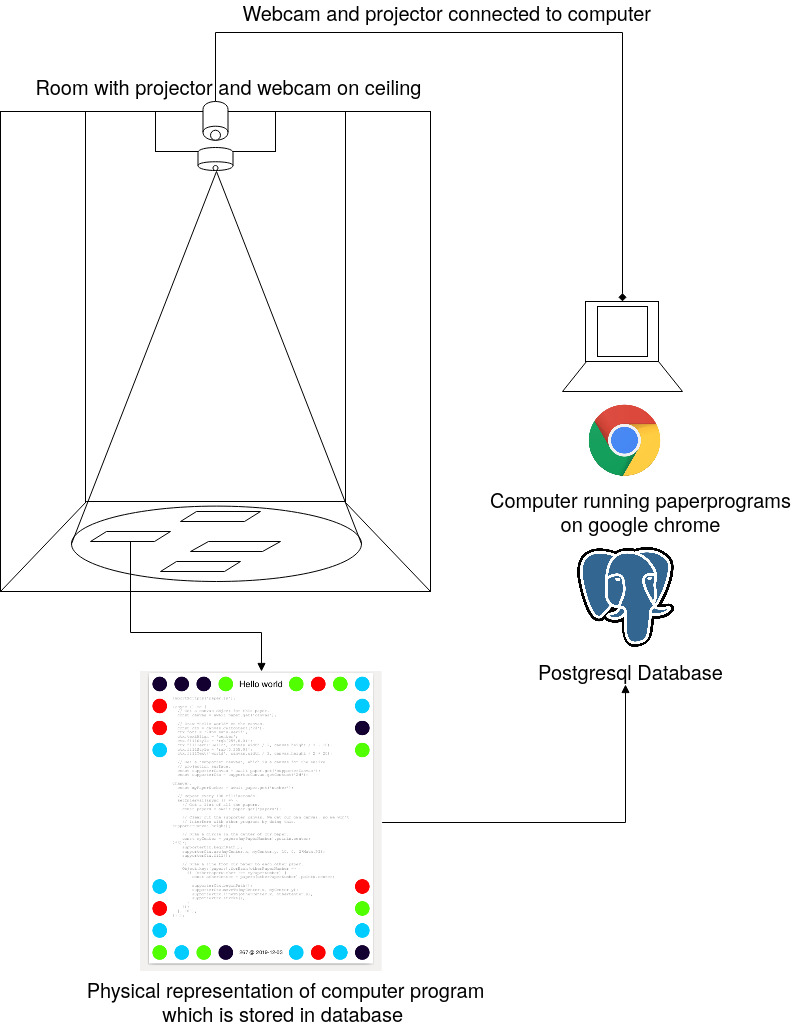
\includegraphics[width=15cm]{assets/pp-diag.png}
\caption{The initial physical schema, using \emph{Paperprograms}, a browser-based partial clone of Dynamicland \label{pp-schema}}
\end{figure}



\section{Paper programs - open source}
\label{sec:orga8cea4f}

\section{Sage digital research}
\label{sec:org0d3c0aa}

\section{Design of everyday things?}
\label{sec:orga1df800}

\section{Nielsen: augmenting ltm and using ai to augment human-i}
\label{sec:org5ea291f}

\section{mental and physical health implications of contemporary computing ? Are they really quite minor?}
\label{sec:orgf89ecc9}

\section{Computational creativity?}
\label{sec:orgc81e7e7}

\begin{enumerate}
\item Open source
\label{sec:org87da904}

\item alex mclean thesis
\label{sec:orgb3a7f7d}

\item 
\label{sec:org2243d13}
\end{enumerate}

\chapter{Specification and context}
\label{sec:org62455f8}
\chapter{Project in depth}
\label{sec:orgf8dcba2}

See system schema Fig.  \ref{system-schema}

\begin{figure}[htbp]
\centering
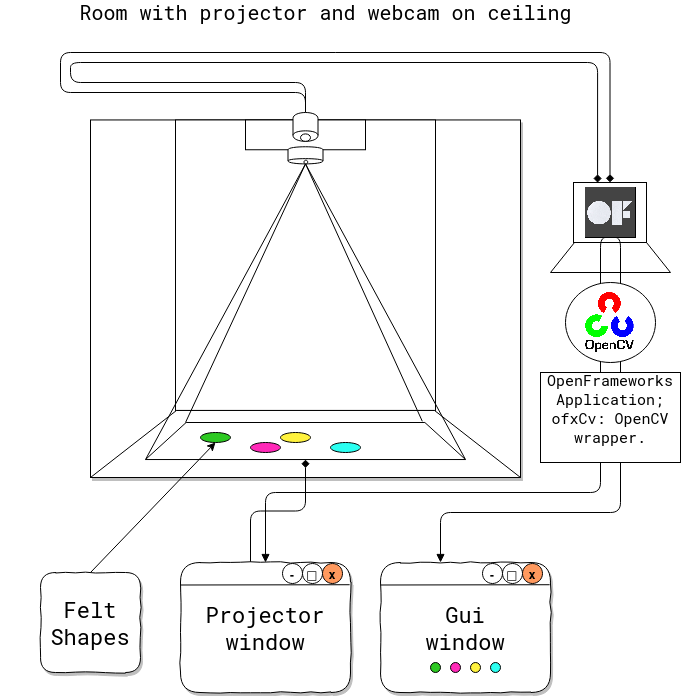
\includegraphics[width=.9\linewidth]{assets/project-schema-final.png}
\caption{System schema \label{system-schema}}
\end{figure}
\chapter{Creative process}
\label{sec:orga3e67eb}
\chapter{Debugging and problem solving}
\label{sec:org3280de0}
\chapter{Evaluation and Conclusions}
\label{sec:org707b8bd}
\bibliographystyle{ieeetr} 
\bibliography{references}
\end{document}
